% Joaquin Matres
%%%%%%%%%%%%%%%%%%%%%%% preamble %%%%%%%%%%%%%%%%%%%%%%%%%%%
\documentclass[10pt,letterpaper]{article}
\usepackage{opex3}
\usepackage{amsmath}

\usepackage{color}
\newcommand{\comment}[1]{\textcolor{red}{#1}}
 %\usepackage{ae} %%for Computer Modern fonts

%%%%%%%%%%%%%%%%%%%%%%% begin %%%%%%%%%%%%%%%%%%%%%%%%%%%%%%
\begin{document}

%%%%%%%%%%%%%%%%%% title page information %%%%%%%%%%%%%%%%%%
\title{Ultrafast nonlinear effects in amorphous silicon waveguides}
%\title{Low carriers silicon nanocrystal-based horizontal slot waveguide}
\author{J. Matres$^{*,1}$, G. C. Ballesteros$^1$, P. Gautier$^2$, J-M F\'ed\'eli$^2$, J. Mart\'i$^1$ and C. J. Oton$^1$} % J. Mart\'i$^1$,
\address{$^1$ Nanophotonics Technology Center, \\ Universidad Polit\'ecnica de Valencia, Camino de Vera s/n, 46022, Valencia, Spain\\
$^2$CEA LETI, Minatec Campus, Grenoble 38054, France}
\email{$^*$joamatab@ntc.upv.es}


%%%%%%%%%%%%%%%%%%% abstract and OCIS codes %%%%%%%%%%%%%%%%
%% [use \begin{abstract*}...\end{abstract*} if exempt from copyright]

\begin{abstract}
We present the characterization of the nonlinear dynamics of a CMOS-compatible amorphous silicon waveguide, where the temporal phase and amplitude response are simultaneously monitored. Results are compared with regular silicon--on--insulator (SOI) waveguides. A higher nonlinear coefficient together with lower two-photon absorption yields to a 8 times higher figure of merit, allowing low--power low--carrier devices not limited in speed by carrier recombination. Measurements are complemented with split-step simulations.
\end{abstract}

%The low power needed to exploit nonlinear effects frees future devices from carrier effects and time limitations imposed by their recombination. Measurements are complemented with split-step simulations.
%The low power needed to exploit nonlinear effects frees future devices from carrier generation and time limitations they impose with their recombination.
%The low power needed to exploit nonlinear effects reduces carrier generation and effects that hinder the speed of optical devices
%and the speed limitation introduced by their recombination.
%the recombination times
%future devices from carrier generation and time limitations they impose with their recombination.
%imposed by their recombination. Measurements are complemented with split-step simulations.

%We present the characterization of the nonlinear dynamics of a CMOS-compatible amorphous silicon waveguide, where the temporal behavior of the phase and amplitude of the nonlinear response are simultaneously monitored. Results are compared with regular Silicon--on--insulator (SOI) crystalline silicon waveguides. A higher nonlinear coefficient together with lower two-photon absorption yields to a 8 times higher figure of merit. Low power needed to exploit nonlinear effects frees future devices from carrier effects and time limitations imposed by their recombination. Measurements are complemented with split-step simulations.

\ocis{(190.0190) Nonlinear optics; (130.0130) Integrated optics; (320.0320) Ultrafast optics; (160.4330) Nonlinear optical materials.}

%(220.0220) Optical design and fabrication; (230.5750) Resonators; (230.3990) Microstructure devices; (250.5300) Photonic Integrated Circuits.}

%%%%%%%%%%%%%%%%%%%%%%% References %%%%%%%%%%%%%%%%%%%%%%%%%

\bibliographystyle{osajnl}
\bibliography{/home/joaquin/Documents/library}


%%%%%%%%%%%%%%%%%%%%%%%%%%%
%%%%%%%%           Introduction           %%%%%%
%%%%%%%%%%%%%%%%%%%%%%%%%%%
\section{Introduction}
%Nonlinear silicon-based photonic devices can introduce key functionalities for on-chip optical signal processing and routing. In the last years, many different nonlinear silicon devices have been reported, such as all-optical modulators~\cite{Almeida2004a}, wavelength converters~\cite{Lee2009}, demultiplexers~\cite{Koos2009}, etc. These nonlinear devices can be based either on free carriers or on the bound-electron Kerr coefficient. In pure silicon waveguides, the Kerr effect is usually hindered by more intense and longer-lasting free-carrier dispersion (FCD). However, it is more desirable to exploit the Kerr effect, as its temporal response is instantaneous (no speed limitation) and it enables parametric conversion and amplification. In order to increase the Kerr coefficent and reduce carrier effects in silicon waveguides we use amorphous silicon waveguides, with high nonlinear coefficient \cite{Narayanan2010} and low TPA thanks to its wider band-gap \cite{OLeary1997}.
%these material involve CMOS processes and as 
%impose strict temperature limitations

Silicon photonics is a technology that is becoming competitive with alternative technologies in photonics, being its high integrability and low cost the most appealing features. Nonlinear silicon photonics is a very active research line, as devices with all-optical functionality could boost their speed with respect to their electrically-controlled counterpart. Many different nonlinear devices have been reported in the last years, such as all-optical modulators,~\cite{Almeida2004a} wavelength converters,~\cite{Lee2009}, etc. \cite{Matres:12}

%All of them can be easily integrated into new devices within a small area thanks to the high refractive index of silicon. However such optical devices have been limited by the carrier dispersion and absorption effects, with a recombination time in the order of nanoseconds. Therefore, when carriers are generated they hinder all-optical devices speed below Gb/s.

All of them can be easily integrated into new devices within a small area thanks to the high refractive index of silicon. However such optical devices have been limited by the carrier dispersion and absorption effects, with a recombination time in the order of nanoseconds. 

Amorphous silicon has been demonstrated to have a high nonlinear coefficient \cite{Narayanan2010} and low TPA thanks to its wider band-gap \cite{OLeary1997}. This could boost the speed of new devices working at low powers at which few carriers are generated. Moreover amorphous silicon is a material that can be easily grown, and as it doesn't require high annealing temperatures, will allow to integrate optical devices and interconnects not affecting previous circuits on the chip.




%%%%%%%%%%%%%%%%%%%%%%%%%%
%%%%%%     Experiment      %%%%%%%%%%%
%%%%%%%%%%%%%%%%%%%%%%%%%%
\section{Fabrication}
Starting with bulk wafers oxidized with 3~$\mu \mathrm{m}$ thickness, a hydrogenated amorphous silicon layer of 253~nm was deposited by Plasma-enhanced chemical vapor deposition (PECVD) at 350\textcelsius. Waveguides were patterned using DUV lithography and HBr Reactive-ion etching, then covered with 1.5~$\mu \mathrm{m}$ m thick silica. Waveguides of 475~nm width and 10~mm length were fabricated and light was coupled horizontally using lensed fibers.

On the other hand, SOI waveguides were also fabricated for comparison. These were processed from SOI wafers with 220~nm Si thickness, patterned with deep-UV lithography and covered with silica after the etching process. Their dimensions were  445$\times$220~nm  for transverse-electric (TE) polarization and 485$\times$220~nm for transverse-magnetic (TM) polarization. Total length was 25~mm and light was coupled through grating couplers.

Figure \ref{fig:sem} shows scanning electron microscopy (SEM) micrographs of the facets. Propagation and coupling loss were measured by characterizing waveguides of different lengths (results are shown in Table \ref{table:results}). 


%Then using DUV lithography and HBr RIE etching waveguides were formed and covered with $1.5\mu m$ thick silica.

\begin{figure}[htb]
    \centering
    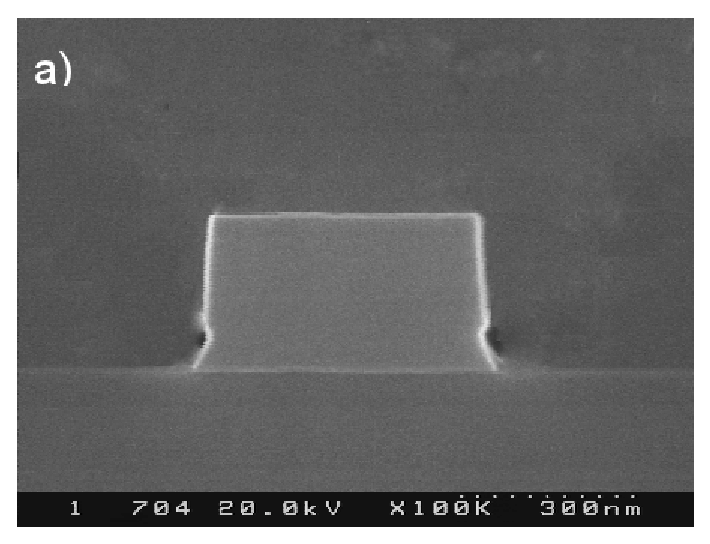
\includegraphics[width=0.32\textwidth]{p13_4}
    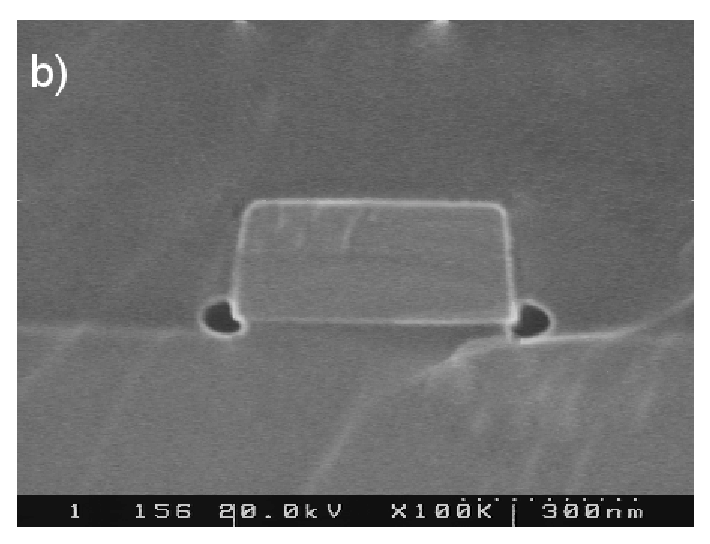
\includegraphics[width=0.32\textwidth]{semTM_4}
    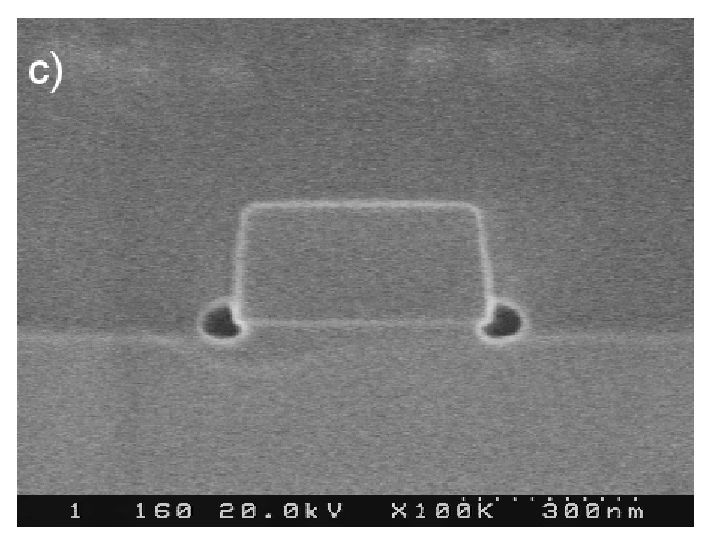
\includegraphics[width=0.32\textwidth]{semTE_2}
    \caption{SEM images of the amorphous silicon (a), TM SOI (b) and TE SOI (c). Air bubbles visible in the SOI samples were generated during facet preparation with HF to increase SEM contrast.}
    \label{fig:sem}
\end{figure}


\section{Time-resolved measurements}
The amorphous silicon waveguide characterized in this paper was 10mm long, where the TM polarization mode was excited. We characterize the samples with a time-resolved phase-sensitive technique similar to the one described in \cite{Vallaitis2008}. In this technique, we divide a 1ps laser pulse into three pulses, one of them intense (pump) and two identical weak ones (a reference and a probe). Then we combine the pump very close to the probe, changing their separation with a variable delay line. Finally the amplitude and phase of the probe is monitored as a function this delay by using a lock--in amplifier.

\begin{figure}[htb]
    \centering
    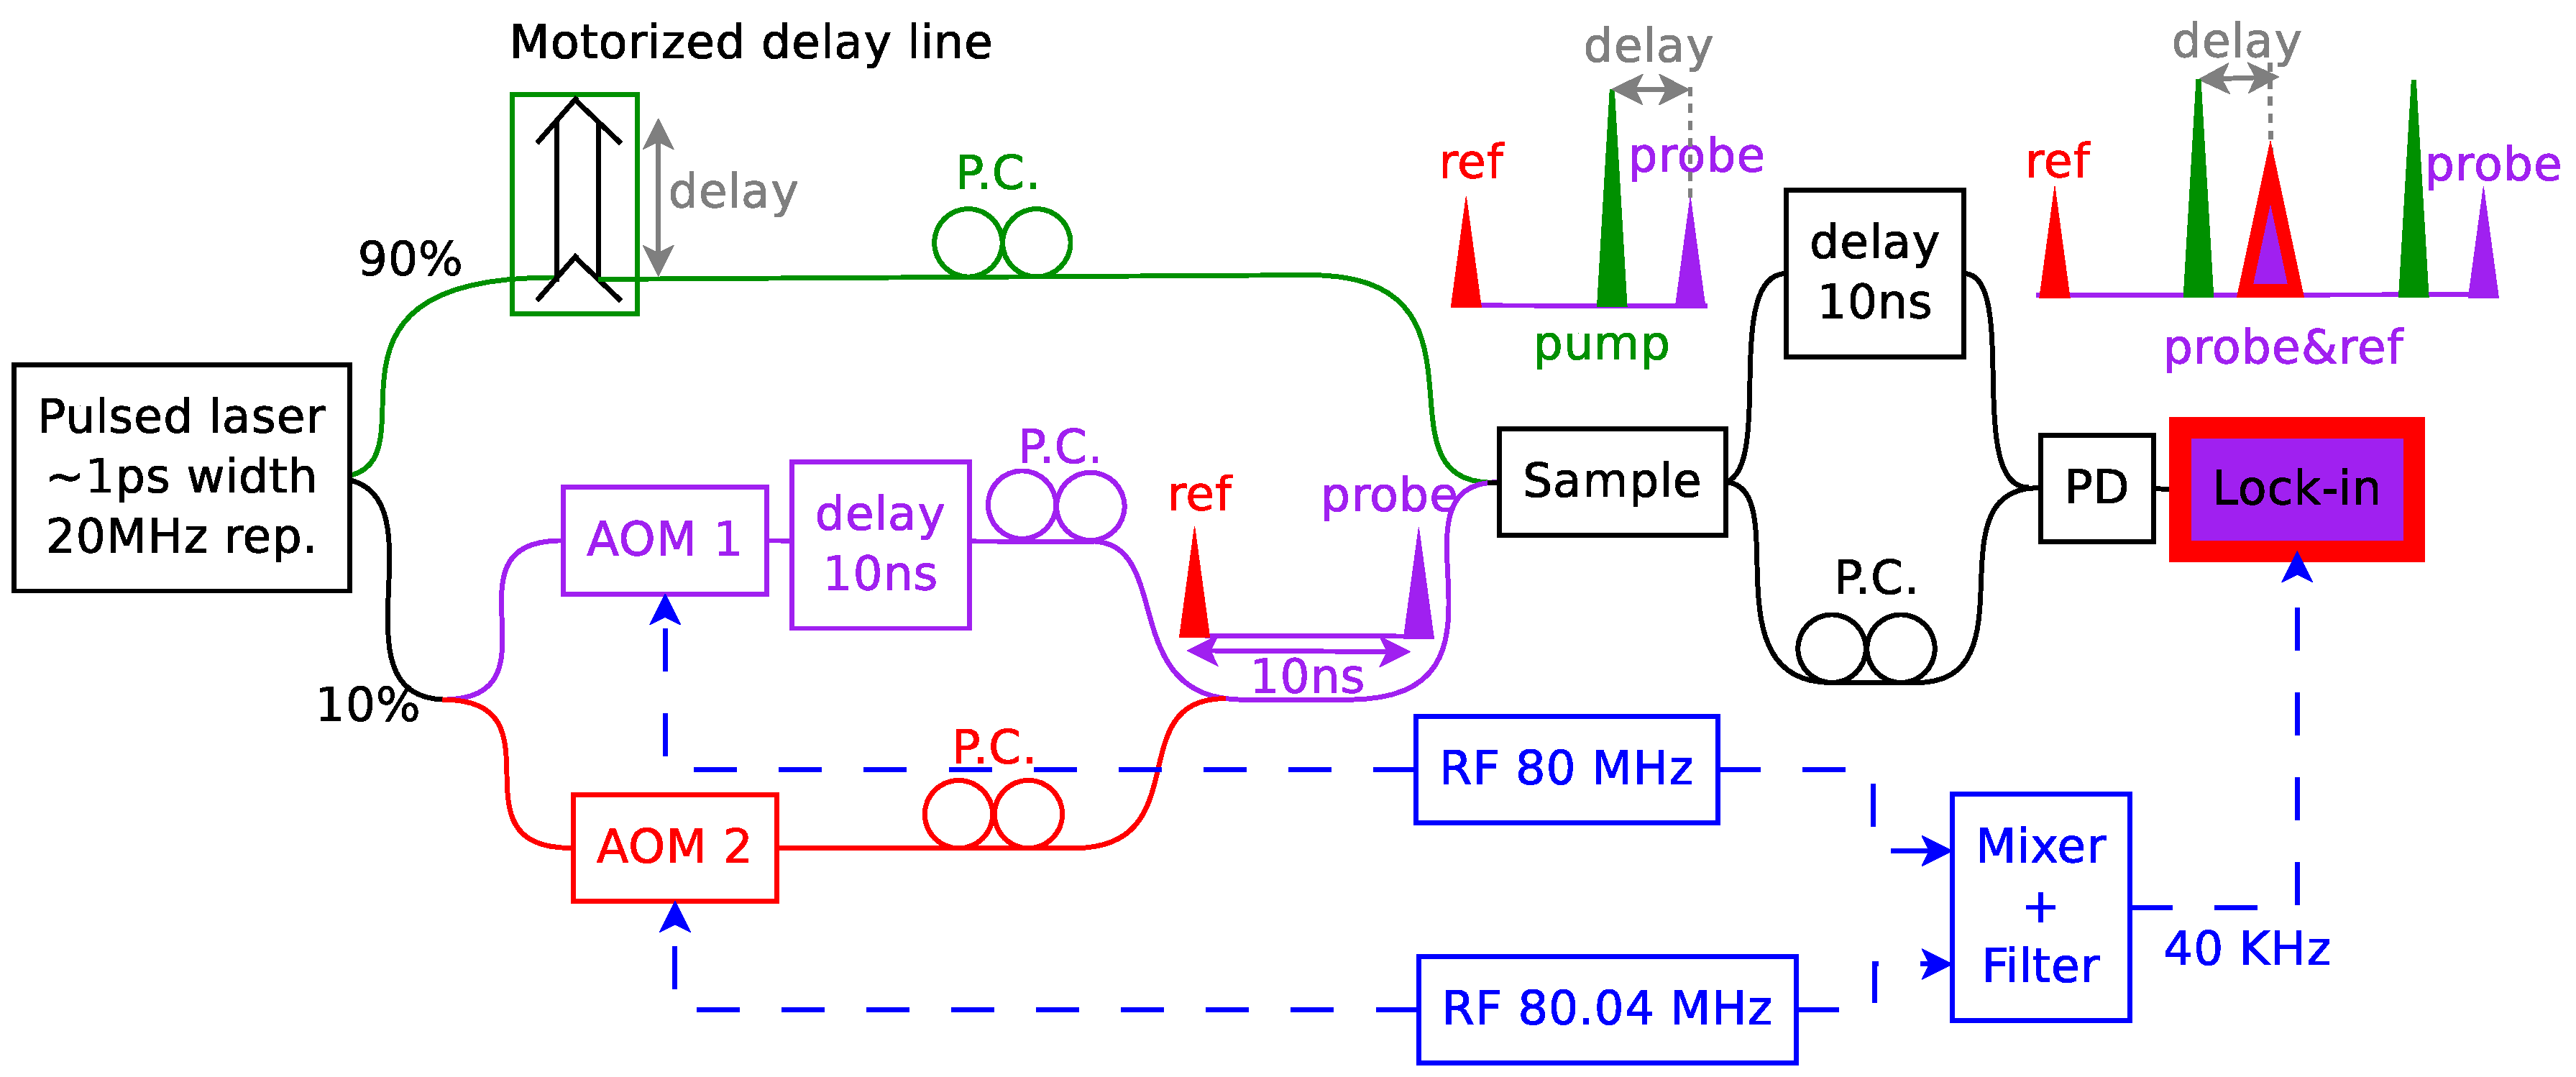
\includegraphics[width=1.0\textwidth]{timeResolved9}
    \caption{Time resolved characterization setup. PD: photodiode, PC: polarization controller, AOM: acousto-optic modulator.}
    \label{fig:setupTimeRes}
\end{figure}


In Fig. \ref{fig:timeResolvesMeasurements} we observe both Kerr and carrier effect in the TM amorphous silicon compared to SOI TM and TE strip waveguides. They produce opposite phase shifts because Kerr produces an increase in refractive index ($ \Delta n > 0 $) and carriers decrease it ($ \Delta n < 0 $).  The dynamics of each of these processes is also very different. During the pump pulse, an instantaneous phase change is due to Kerr effect, together with an amplitude decrease. This decrease is due to cross-absorption modulation (XAM), which consists of a two-photon absorption (TPA) process where one of the photons comes from the pump and the other one comes from the probe. Once the pump pulse is gone, there is a phase response with opposite sign that remains for all the measurement range. This is due to the carrier plasma effect, also known as free-carrier dispersion (FCD). 


%In Fig. \ref{fig:timeResolvesMeasurements} one can observe both Kerr and carriers effect in a regular TM strip waveguide compared to our waveguide for similar values of peak power in waveguide. They produce opposite phase shifts because Kerr produces an increase in refractive index ($ \Delta n > 0 $) and carriers decrease it ($ \Delta n < 0 $).  The dynamics of each of these processes is also very different. During the pump pulse, we can see an instantaneous phase change due to Kerr effect, together with an amplitude decrease. This decrease is due to cross-absorption modulation (XAM), which consists of a two-photon absorption (TPA) process where one of the photons comes from the pump and the other comes from the probe. Once the pump pulse is gone, there is a phase response with opposite sign that remains for all the measurement range. This is due to the carrier plasma effect, also known as free-carrier dispersion (FCD). 
%It is worth noting that a phase shift higher than $\pi/2$ is achieved with the highest pump pulse.

The measurement of the amplitude attenuation due to XAM is affected by the artifact reported in \cite{Vallaitis2009}, where the abrupt phase changes create a frequency shift in the probe signal modifying the signal detected in the lock-in amplifier. For this reason, in order to obtain a reliable measurement of TPA, we performed nonlinear transmission experiments which are reported in section~\ref{sec:imGamma}.


%cannot be determined at high peak powers because the abrupt phase changes create a frequency shift in the probe signal modifying the signal detected in the lock-in amplifier. This artifact was also reported in \cite{Vallaitis2009}, so in order to get a more reliable measurement of TPA we performed transmission experiments, which are reported in section~\ref{sec:imGamma}.
%  was  is an artifact of the measurement system, so in order to obtain the TPA we measured losses for different peak powers (See section~\ref{sec:imGamma}). 

%One can calculate the figure of merit (FOM) by using the analysis in Ref. \cite{Vallaitis2009}, for which no estimations of effective area or even peak power are needed. Using the same procedure, we obtained a FOM value of 1,  which is a factor of 2 and 4 higher than TM and TE strip waveguides. 

%In order to compare this result, we also measured a pure silicon sample of dimensions 220x500~nm, and the FOM was 0.1,.



%However, there is also a power penalty due to XAM. In order to quantify the balance between XAM and Kerr effect, one can calculate the figure of merit (FOM) by using the analysis in Ref. \cite{Vallaitis2009}, for which no estimations of effective area or even peak power are needed. Using the same procedure, we obtained a FOM value of 0.4. 
%In order to compare this result, we also measured a pure silicon sample of dimensions 220x500~nm, and the FOM was 0.1, which is a factor of 4 lower.
%\cite{Lin2007}



\begin{figure}[htb]
    \centering
    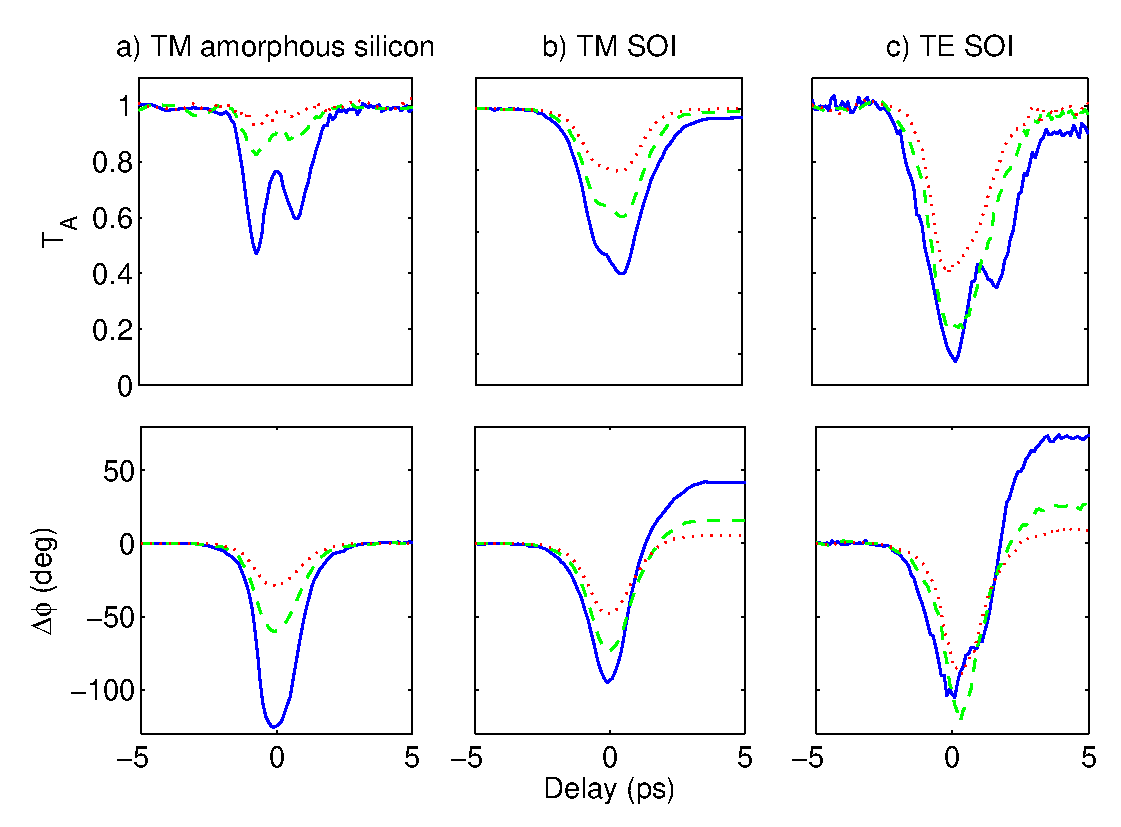
\includegraphics[width=0.68\textwidth]{timeResAmorfoTm10mmP13b_1w_0p5_0p25_0p125_amp_SOI_2}
    \caption{Time resolved measurements for different peak powers in waveguide. a) 0.8W (---), 0.4W (-~-), 0.2W ($\cdot~\cdot$) b) 6W (---), 3W (-~-), 1.5W ($\cdot~\cdot$) c) 3W (---), 1.5W (-~-), 0.75W ($\cdot~\cdot$) }
    \label{fig:timeResolvesMeasurements}
\end{figure}



\section{Nonlinear loss measurements: Im\{$ \gamma $\}}
\label{sec:imGamma}
Two-photon absorption is a well-known process in silicon waveguides. In a waveguide, we can consider it as the imaginary part of the gamma coefficient of the waveguide by using this differential equation:

\begin{equation}
 \frac{dP}{dz} = -\alpha_0 P(z) - 2|Im(\gamma)| P(z)^2 
\label{eq:differentialTPA}
\end{equation}

where P is the signal power through the waveguide, $\alpha$ is the linear loss of the waveguide, and $Im(\gamma)$ is the imaginary part of the $\gamma$ coefficient (we use the absolute value because $Im(\gamma)$ is negative, but we want to stress its loss character in the equation with a negative sign). 

The solution of the differential equation shown in Eq.~\ref{eq:differentialTPA} after a distance $L$ is given by:

\begin{equation}
 P(L) = \frac{e^{-\alpha_0 L}}{1+2|Im(\gamma)| L_{eff} P_0} P_0
\end{equation}

where $P_0$ is the input power in the waveguide. Therefore the relationship between the transmission at high power ($T_{HP} = P(L)/P_0 $) and the transmission at low power ($T_{LP} = e^{-\alpha_0 L} $) represents only the nonlinear loss $T_{NL}$:

\begin{equation}
 T_{NL}^{-1} = \frac{T_{LP}}{T_{HP}} = 1+2|Im(\gamma)| L_{eff} P_0
\label{eq:transmissionLinear}
\end{equation}

which is a linear function on $P_0$. The slope of the curve can give us the two-photon absorption coefficient of our waveguide as in \cite{Vallaitis2009}.
However, this equation is only valid for instantaneous transmission values. When a pulsed signal is sent, and the transmission is averaged over time, the measured transmission would be the integral of the output, which we can define as

%If one sends a pulsed signal, the equation is still correct for every instantaneous moment, but not correct for the overall transmission energy of the pulse.
%If one defines the energy transmission of a pulse $ \tilde{T} $ as the amount read by a power meter, one has to integrate the power along the whole pulse duration:

\begin{equation}
 \tilde{T}  = \frac{\int P(t,L)dt}{\int P_0(t)dt}
\end{equation}

where $\tilde{T}$ represent the averaged transmission of a pulsed signal with an input shape given by $P_0(t)$. With this definition, the ratio with the transmission at low power would be given by:


%\begin{equation}
 %\tilde{T} (L)^{-1} = \frac{\int P_0(t)dt}{\int P(t,L)dt} = \frac{\int P_0(t)dt} {e^{-\alpha L} \int \frac{P_0(t)}{1+2|Im(\gamma)| L_{eff} P_0(t)} dt}
%\end{equation}

\begin{equation}
\tilde{T}_{NL}^{-1} = \frac{\tilde{T}_{LP}}{\tilde{T}_{HP}} = \frac{\int P_0(t)dt}{\int \frac{P_0(t)}{1+2|Im(\gamma)| L_{eff} P_0(t)} dt}
\label{eq:transmissionIntegral}
\end{equation}


which depends on the actual pulse shape $P_{0}(t)$ that is introduced. If the pulsed signal has a rectangular shape, one can use Eq.~\ref{eq:transmissionLinear}, but if the shape is different, the integral in Eq.~\ref{eq:transmissionIntegral} must be solved, as the result differs significantly. The reason for this variation is the fact that the flanks of the pulse are not affected as hardly by TPA as the peak. Therefore, the overall energy transmission is higher than for the case of cw excitation. For the particular case of a $sech^2$ shape, which corresponds to the output of our laser, the result of  Eq.~\ref{eq:transmissionIntegral} is given by:

% One can calculate analytically how much this transmission is for different typical pulse shapes.

%We assume a hyperbolic secant pulse, typical for solitons, which is the shape of our femtosecond fiber laser $  P_0(t) = P_{0 peak}~\mathrm{sech}^2 (\frac{t}{\tau}) $. Solving Eq.~\ref{eq:transmissionIntegral} for the hyperbolic secant is not trivial. After some algebraic manipulation and using some properties of inverse hyperbolic trigonometric functions, one can extract the analytical result, which is:<

%\begin{equation}
% P_0(t) = P_{0 peak}~sech^2 \frac{t}{\tau}
%\end{equation}



\begin{equation}
\tilde{T}_{NL}^{-1} = \frac{\tilde{T}_{LP}}{\tilde{T}_{HP}} \bigg|_{sech^2~shape}  = \frac{\sqrt{\delta}\sqrt{\delta + 1}}{\ln(\sqrt{\delta}+\sqrt{\delta+1})} ~~\mathrm{where}~~  \delta = 2|Im(\gamma)| L_{eff} P_{0 peak}
\label{eq:transmissionHypSecant}
\end{equation}

%for $ \delta = 2|Im(\gamma)| L_{eff} P_{0 peak} $

%\begin{figure}[htb]
 %   \centering
  %  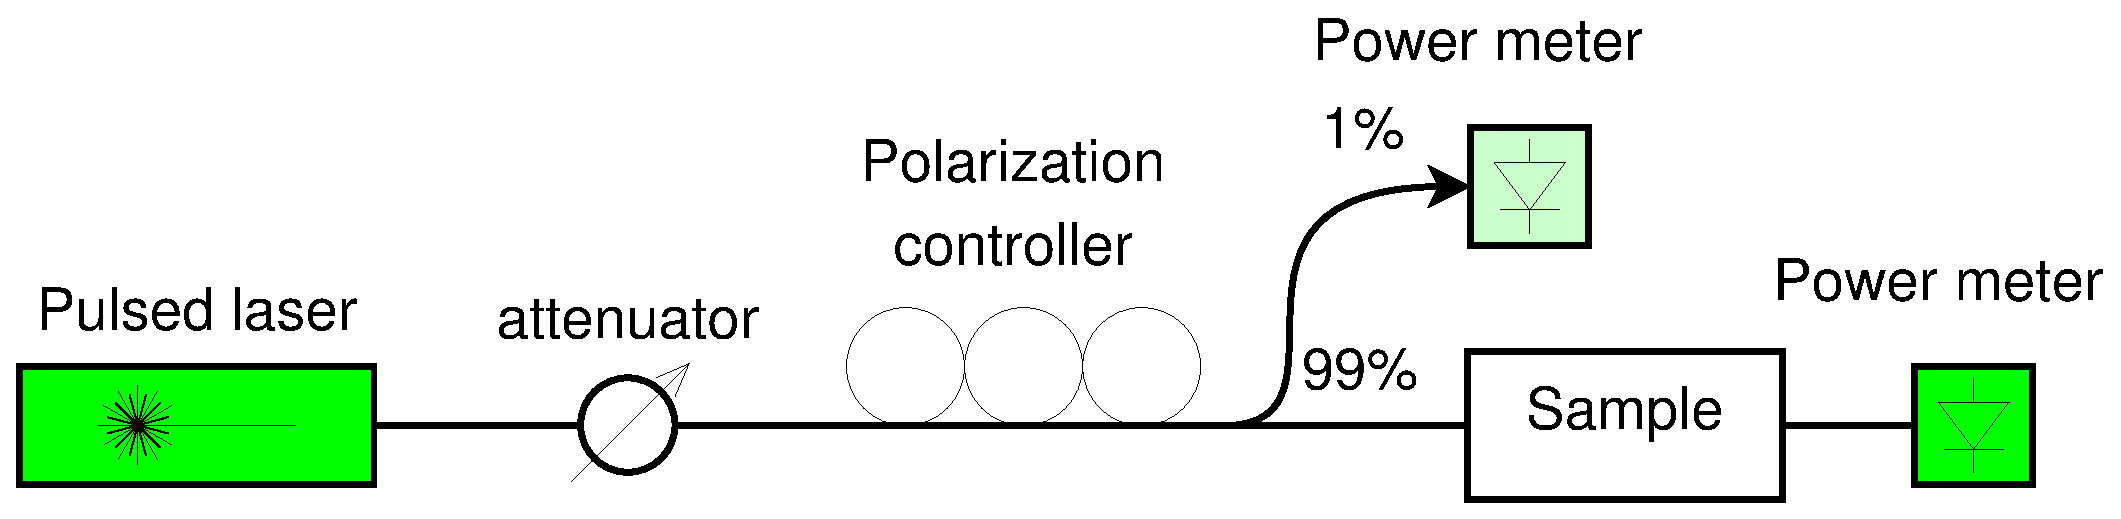
\includegraphics[width=1.0\textwidth]{imGammaFit}
   % \caption{Absorption characterization setup.}
    %\label{fig:setupImGamma}
%\end{figure}


We measured this parameter with a power meter using a picosecond laser at a wavelength of 1539~nm, and a variable attenuator. The results are shown in Fig.~\ref{fig:imGammaSamples}, where the curves were fitted to Eq.~\ref{eq:transmissionHypSecant} in order to extract the parameter $Im(\gamma)$ used in the simulations. The results of the fits are shown in Table~\ref{table:results}.

\begin{figure}[htb]
    \centering
    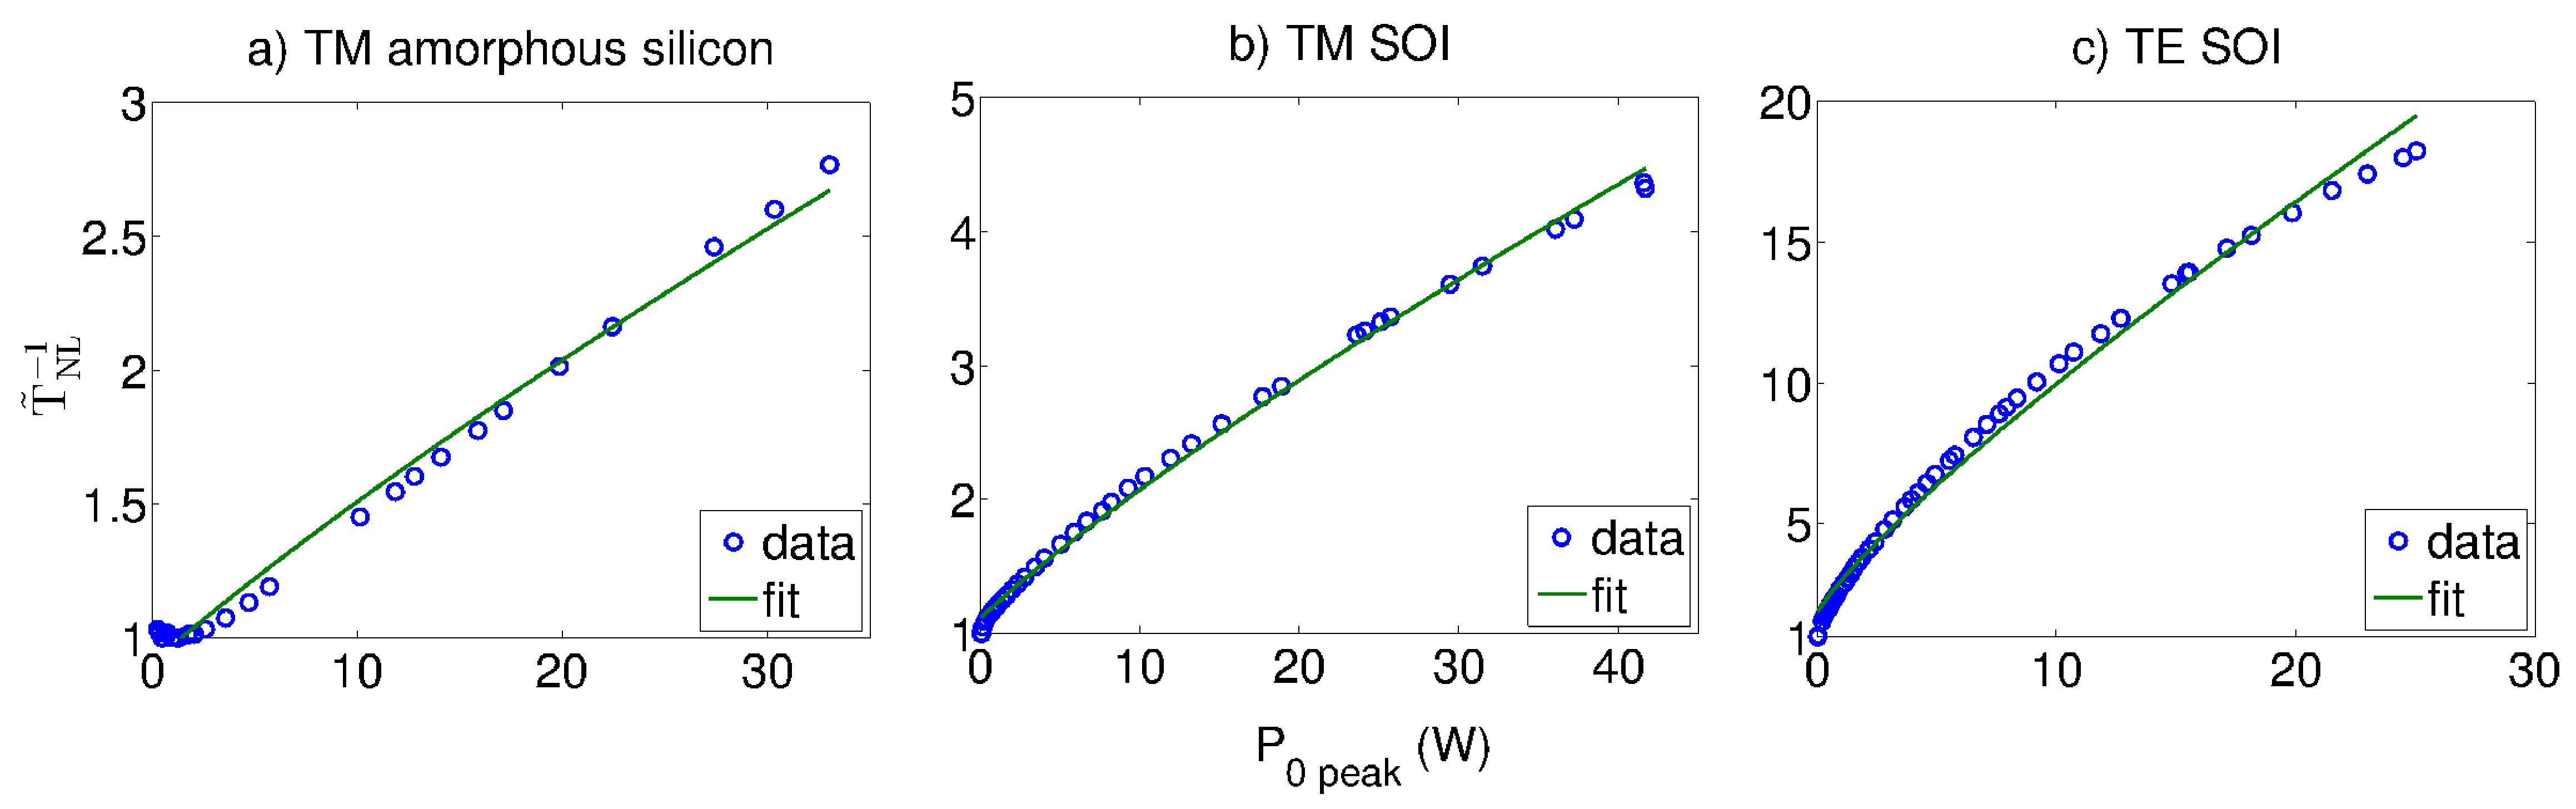
\includegraphics[width=1.00\textwidth]{imGamma_aSi_TM_TE}
    %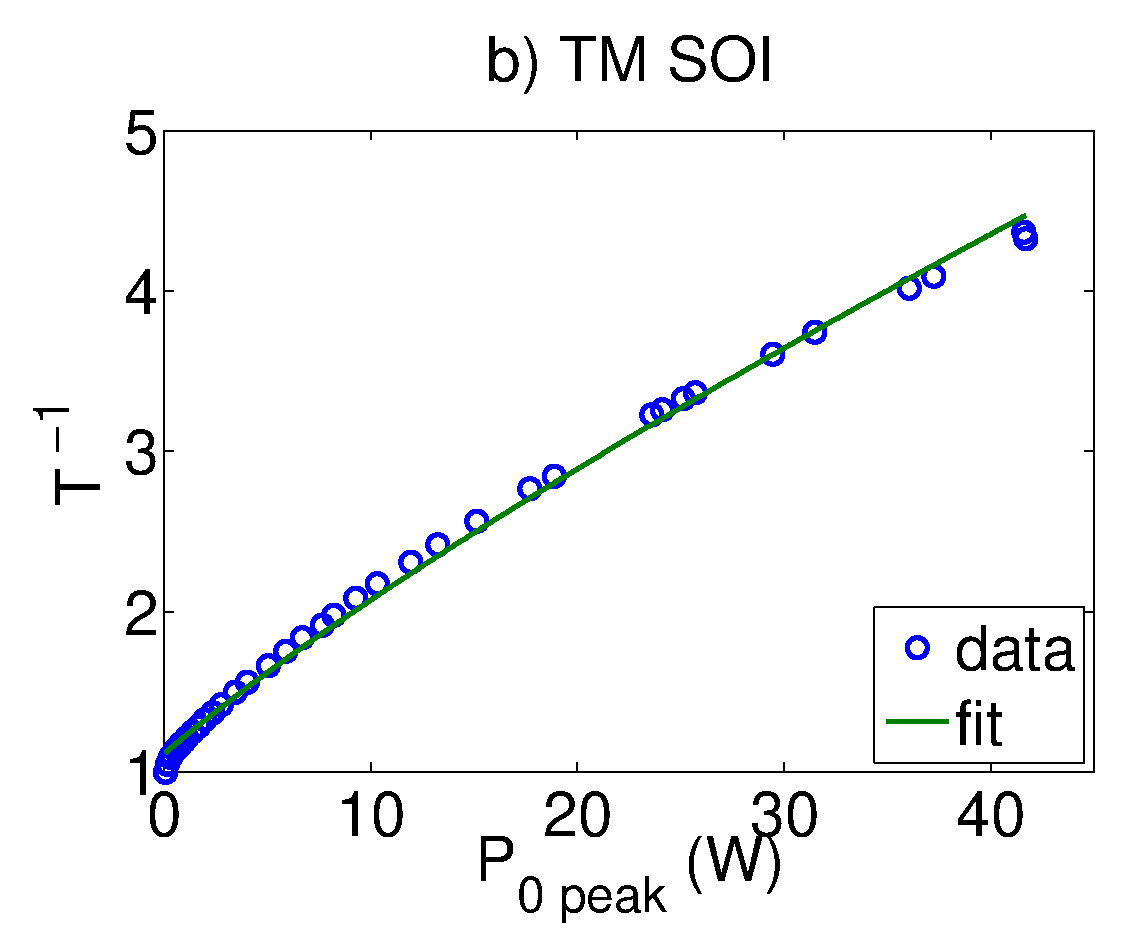
\includegraphics[width=0.32\textwidth]{imGamma_5p4366_V740TM25mm_big30}   
    %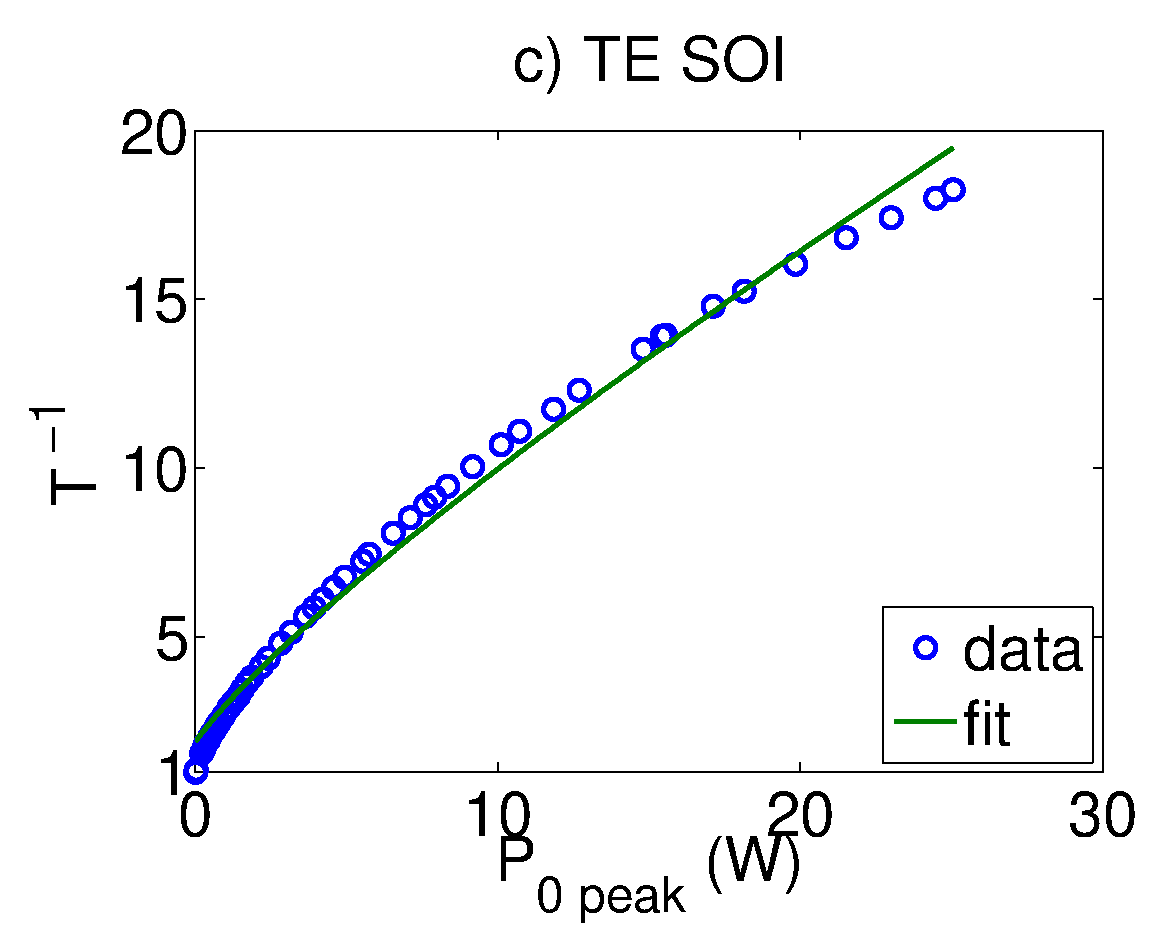
\includegraphics[width=0.32\textwidth]{imGamma_117Wm-1_V740TE25mm_big30}
      \caption{Transmission versus waveguide peak power (note the difference in the y-scale among the three plots). Solid line shows the fit for $ sech^2 $ pulses using Eq.~\ref{eq:transmissionHypSecant}.}
    \label{fig:imGammaSamples}
\end{figure}


\section{Time-resolved simulations}
We used the nonlinear Schr\"{o}dinger equation to simulate the propagation of pump and probe pulses in optical waveguides \cite{Agrawal2001a}. Solving the equation with the symmetrized split-step Fourier method as in \cite{Lin2007}, we cross-check simulations with experimental measurements in Figure~\ref{fig:timeResolvesSimulations}. The output of the simulation is the envelope of the pump, probe and reference pulses, so in order to extract the output of the lock-in amplifier we calculated the overlap integral of the probe and reference pulses:

%we need to combine the last two of them to simulate the value that would be read off the lock-in amplifier. We did this by calculating an overlap integral of probe and reference pulses normalized to the power of the reference pulse. The amplitude (phase) of the integral was used as a measure of the transmission (relative phase) that a lock-in amplifier would output.
%This allow us to make efficient and precise simulations of the propagation 
%and to use the fitting values as a cross-check for the results obtained through other methods. 
%An adapted version of the nonlinear Schr\"{o}dinger equation to simulate the simultaneous propagation of pump and probe pulses in optical waveguides \cite{Agrawal2001a} was used. The equation was solved using the symmetrized split-step Fourier method as described in \cite{Lin2007}. The latter allowed us to make efficient and precise simulations of the propagation and to use the fitting values as a cross-check for the results obtained through other methods. Since the output of the simulator is the envelope of the pump, probe and reference pulses we need to somehow combine the last two of them to simulate the value that would be read off the lock-in amplifier. We did this by calculating an overlap integral of probe and reference pulses normalized to the power of the reference pulse. The amplitude (phase) of the integral was used as a measure of the transmission (relative phase) that a lock-in amplifier would output.


\begin{equation}
        |T_{A}|e^{j\phi} =
        \frac{\int E_{\mathrm{ref}}(\tau) E^*_{\mathrm{probe}}(\tau) ~ \mathrm{d}\tau}
        {\int |E_{\mathrm{ref}}(\tau)|^2~\mathrm{d}\tau}
\end{equation}


%where $T_A$ and $\phi$ are respectively the transmitted amplitude and phase measured in the lock--in amplifier.
where $T_A$ and $\phi$ are the transmitted amplitude and phase measured in the lock--in amplifier.

\begin{figure}[htb]
    \centering
    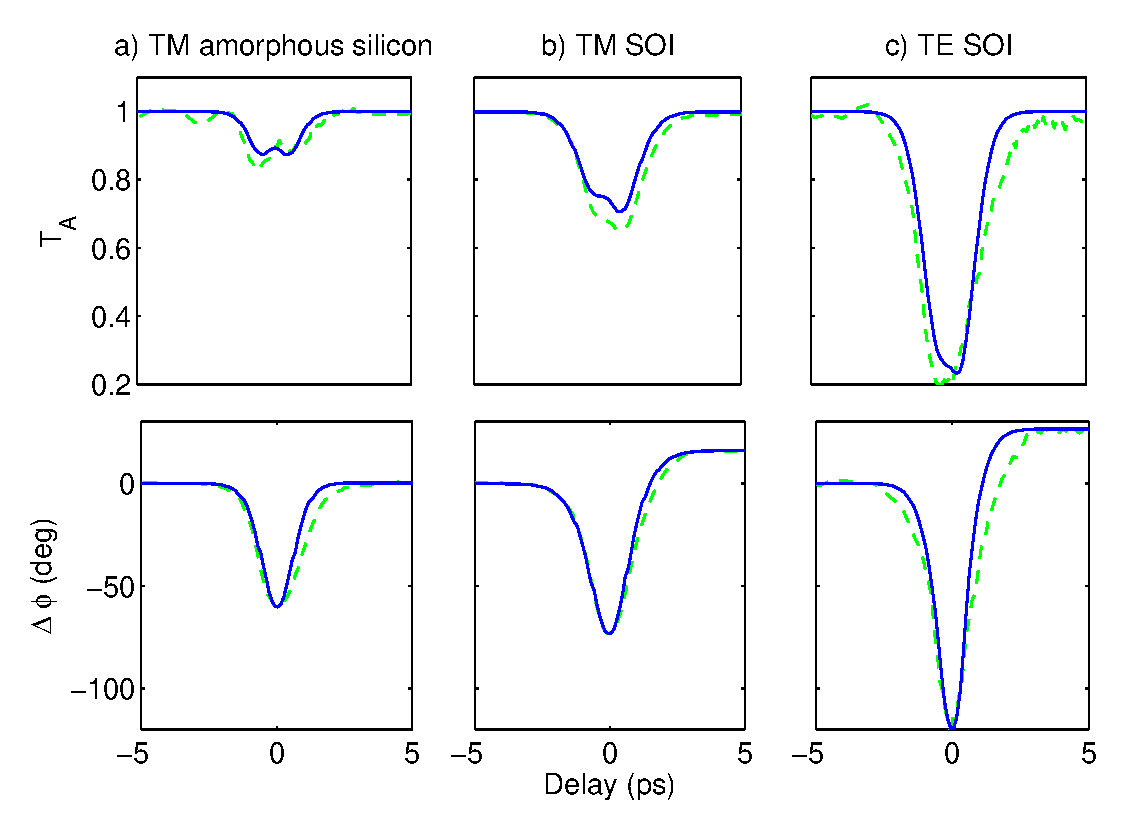
\includegraphics[width=0.68\textwidth]{timeRes_simulations_AmorfoTm10mmP13b_0p5w_SOI_2w__}
    \caption{Time resolved measurements (-~-) and simulations (---) for 0.4W (sample a), 3W (sample b) and 1.5W (sample c) peak power in waveguide.}
    \label{fig:timeResolvesSimulations}
\end{figure}


\section{Results and conclusion}

\begin{table}
\centering
\caption{Extracted linear and nonlinear parameters from the experiment for the three samples: the TM amorphous silicon, the 485$\times$220~nm TM SOI and the 445$\times$220~nm TE SOI waveguide. Dispersion values for SOI waveguides were obtained with the technique shown in paper~\cite{Mas2012} and in the amorphous silicon through four--wave--mixing conversion efficiency bandwidth.}
\begin{tabular}{l|ccc}
\hline
Sample & TM amorphous silicon & TM SOI & TE SOI \\\hline
coupling (dB) & 7.5 & 6 & 6\\
propagation (dB/cm) & 4 & 1.9 & 4.9\\
$L_{eff}$ (mm) & 6.5 & 15.2 & 8.3\\
 Dispersion  (ps/(km$\cdot$nm))   & -6500 & -19800 & -1200\\
  $ Im(\gamma)~(\mathrm{W}\cdot \mathrm{m})^{-1} $     & 5.4 & 5.4 & 68.1\\
    $ Re(\gamma)~(\mathrm{W}\cdot \mathrm{m})^{-1} $        & 332 & 40 & 245\\
$ FOM = \frac{1}{4\pi} \frac{Re\{\gamma\}}{|Im\{\gamma\}|} $  & 4.9 & 0.59 & 0.29 \\
 effective FCD $ \frac{-\sigma_n}{ A_{eff} }~(10^{-15}~\mathrm{m}) $ & 0 & 21 & 28 \\
\hline
\end{tabular}
\label{table:results}
\end{table}




% $  \frac{\sigma_n}{A_{eff}^2} (\mathrm{FCD~per~unit~length})~[\mathrm{m^{-1}}] $  & \textless -0.0034 & -0.0010 & -0.2759 \\
%{Free-carrier absorption (FCA) and dispersion (FCD) for silicon are similar to the ones in paper \cite{Lin2007}.}
%$ \sigma_a~(\mathrm{FCA})~[10^{-17} ~ \mathrm{cm^2}]$   & 1 & 0.5 & 0.5 \\
%TM silicon-nanocrystal-based slot waveguide compared with 443x220 and 487x220nm (TE and TM) silicon strip waveguides. Free-carrier absorption (FCA) and dispersion (FCD) in simulations of the strip waveguides are similar to the ones in paper \cite{Lin2007}.}
%Carriers generated in the TM horizontal 
%Free-carrier absorption (FCA) and dispersion (FCD) are defined and similar to the ones in paper
%*Similar values for the simulations defined in ... were defined and taken from
%Values used for the simulation are similar as the ones defined in




The amorphous silicon waveguide needs a quarter of the power to achieve the same nonlinear effect than the SOI waveguides. Moreover, as its TPA coefficent is also lower, less carriers are generated. This is clear from Fig.~\ref{fig:timeResolvesMeasurements}, and its negligible $\sigma_n$ parameter, defined in \cite{Lin2007} and shown in Table~\ref{table:results}. This would reduce the undesired patterning effects when modulating a real bit pattern. On the other hand, the figure of merit (FOM) that provides the ratio between Kerr effect and TPA is also significantly higher than the SOI waveguides, as shown in Table~\ref{table:results}. The TM mode of the SOI waveguide has a higher FOM than the TE because the TM mode also has more energy in the cladding than the TE mode. These results agree with the ones shown in Ref.~\cite{Vallaitis2009} for a polymer-filled vertical slot; however, our amorphous silicon waveguide, being made of inorganic materials and only requiring CMOS processes, is expected to provide more 
robust and stable material for optical devices. It can also be easily grown through PECVD on chips with circuits already integrated, not needing high annealing temperatures.

In conclusion, ultrafast nonlinear measurements show that amorphous silicon waveguides show much stronger nonlinear effect and carrier generation through TPA than regular SOI waveguides. This makes the amorphous silicon, a material better suited for CMOS-compatible high-speed all-optical processing devices than simple SOI waveguides as it has a figure of times 8 times larger.



%devices with less temperature constraints being able to grow amorphous silicon through PECVD on chips already processed.
%The first significant result is the fact that amorphous silicon waveguides need less than a quarter of the power to achieve the same nonlinear effect than SOI waveguides. Moreover, as the TPA coefficent is also lower, weaker carrier effect than in SOI waveguides were observed. This is clear from Fig.~\ref{fig:timeResolvesMeasurements}, and also from the $\sigma_n$ parameter, defined in \cite{Lin2007} and shown in Table~\ref{table:results}.
%This considerably reduces the undesired patterning effects when modulating a real bit pattern. On the other hand, the figure of merit (FOM) that provides the ratio between Kerr effect and TPA is also significantly higher than the SOI waveguides, as shown in Table~\ref{table:results}. The TM mode of the SOI waveguide has a higher FOM than the TE because the TM mode also has more energy in the cladding than the TE mode. These results agree with the ones shown in Ref.~\cite{Vallaitis2009} for a polymer-filled vertical slot; however, our system, being made of inorganic materials and only requiring CMOS processes, is expected to provide more robust and stable devices with less temperature constraints being able to grow amorphous silicon through PECVD on chips already processed.
%In conclusion, TM horizontal slot waveguides with silicon nanocrystals could be exploited for nonlinear applications thanks to their high nonlinear coefficient not being hindered by the free-carrier limitations. When carrier effects are involved, the speed in optical devices is limited by their recombination time, which is usually in the order of 1\,ns. However with the time resolved measurements we have observed half free-carrier-absorption (FCA) and an order of magnitude lower free-carrier-dispersion (FCD) thanks to the geometry of the slot waveguide. This could be exploited for high speed optical devices with the advantage of being CMOS-compatible.


\section*{Acknowledgments}
We acknowledge Spanish Ministry of Science and Innovation SINADEC(TEC2008-06333) and PROMETEO/2010/087 NANOFOTONICA projects, and Universidad Polit\'ecnica de Valencia for PAID 2011/1914 and J. Matres' doctoral grant.


%We acknowledge financial support from the EU project PHOLOGIC (FP6-IST-NMP-017158), the Spanish Ministry of Science and Innovation through contracts SINADEC (TEC2008- 06333) and DEMOTEC (TEC2008-06360). Joaquin Matres is supported by a doctoral grant of the Universidad Polit\'ecnica de Valencia.
\end{document} 
